\chapter{Analysis Strategy and Event Selection}\label{chapter:tzq-search}
The following three chapters of this thesis describe the search for the production of a single top quark in association with a Z boson using the dilepton final state with 35.9\fbinv of proton-proton collision data at $\sqrt{s} = 13\TeV$ collected by the CMS experiment during 2016.

While the dilepton final state allows for the full reconstruction of all the particles involved, including the top quark, the presence of two leptons and multiple jets is identical to the final states of a large number of background processes.
Consequently, as each of these backgrounds have cross sections many orders of magnitude larger than that for tZq, the signal region will inevitably be background dominated.

Therefore, the analysis was designed to ensure that the backgrounds are understood and constrained as far as possible and to have the highest possible acceptance of the signal in order to maximise the expected tZq yield.
To further enhance the separation of the signal from the background processes, a multivariate analysis is performed and is described in Section~\ref{sec:mvas}.

This chapter describes the event selection criteria used for the signal and control regions used in this search, the blinding method used, and the background processes that were considered.
The selection criteria for the physics objects described in Sections~\ref{sec:signalRegion}-\ref{sec:controlRegions} are defined in detail in Section~\ref{sec:physicsObjects}.

\section{Signal Region}\label{sec:signalRegion}
At leading order, the final state produced by the signal process consists of a top quark, a recoil quark and a Z boson, as illustrated in Figure~\ref{fig:feyn_tZq}.
The top quark decays to a b-quark almost 100\% of the time, with the W boson required to decay hadronically.
As the Z boson is required to decay leptonically, the final state objects of interest consist of two leptons (electrons or muons) that are compatible with a Z boson decay, four jets, one from the top quark decay (which must be b-tagged), two from the W boson, and the recoil jet.

Exactly two leptons are required to pass high purity (tight) identification and isolation criteria with no additional leptons which have passed the most efficient (veto/loose) identification and isolation criteria.
These criteria ensure that there is a low lepton misidentification acceptance rate and a high rejection efficiency of events containing a differing number of leptons of either flavour or that were not produced from a W or Z boson decay.

The presence of a Z boson in the final state means that the two leptons selected must be consistent with being from a Z boson decay.
Thus, the leptons must have the same flavour and opposite charge and an invariant mass that is within $20\GeV$ of the measured Z boson mass of 91.2\GeV~\cite{Tanabashi:2018oca}.
This mass window was chosen as was sufficiently wide to account for detector resolution effects, leading to a high acceptance rate of leptons produced from Z boson decays.

As additional jets may be produced by gluon splitting from by initial or final state radiation the maximum number of jets considered is limited to six.
Thus four to six jets are required to be present, each of which must satisfy $\pT > 30\GeVc$ and $|\eta| < 4.7$ and pass a highly efficient jet identification criteria.

Given the top quark has a near 100\% probability of decaying into a b-quark and a W boson, the event selection requires at least one of the selected jets to be b-tagged and satisfy $|\eta| < 2.7$.
The b-tagging algorithm and selection criteria are described in Section~\ref{subsubsec:bTag}
As the W boson and the recoil quark may also be b-quarks, up to two of the selected jets are allowed to be b-jets.
This limit was chosen as it was found that there was minimal signal (< 1\%) for b-jet multiplicities greater than two which would have been difficult to separate from the large background contributions present.  

With all the jets identified, the W boson candidate constructed from the two jets with the closest invariant mass to the known W boson mass of 80.4\GeVcc~\cite{Tanabashi:2018oca} is considered.
To ensure the two selected jets are consistent with a W boson decay, their invariant mass is required to be within $\pm 20\GeVcc$ of the known W boson mass.
The leading b-jet however, is not considered to have been produced by the W boson decay as the hardest b-jet was found to be predominantly that from the decay of the top quark.

To summarise the complete event selection for the signal region was chosen to be:

\begin{itemize}
\item Exactly two same flavour and opposite sign electrons or muons which pass the tight identification and isolation cuts. The leading and sub-leading electrons must have a $\pT > 35\GeVc (15\GeVc)$ and be within $|\eta| < 2.50$. The leading and sub-leading muons $\pT > 26\GeVc (20\GeVc)$ respectively and be within $|\eta| < 2.4$.
\item  No additional electrons or muons that pass the same kinematic cuts and the veto or loose identification and isolation cuts respectively. 
\item The invariant mass of the two selected leptons must be within $20\GeVcc$ of the known Z boson mass.
\item Four to six jets that pass the jet identification requirements and have a $\pt > 30\GeVc$ and are within $|\eta| < 4.7$.
\item One or two of the selected jets are considered to be b-tagged and are within $|\eta| < 2.4$.
\item The invariant mass of the two jets that are closest to the known W boson mass must be within $20\GeVcc$. The leading b-jet is not considered to have originated from the W boson decay.
\end{itemize}

\section{Control Regions}\label{sec:controlRegions}
For any high energy particle physics analysis lacking a high signal to background ratio, the accurate modelling of its background processes is essential in order to extract the signal yield and make a precise measurement.
As the main challenge in the search for the dilepton final state of the tZq process is the understanding and constraining of its irreducible backgrounds, it is especially important to ensure that the background processes are accurately modelled in simulation.

Therefore, background enriched control regions whose kinematic distributions are similar to the signal region's were constructed and used to check the modelling of the Z+jets and \ttbar production process, as these were anticipated to be the most important background processes.	
Consequently, the control regions for both of these processes had the same trigger, event cleaning, and baseline event selection of two oppositely charged leptons, jet multiplicities and W and Z boson mass selections as the signal region.
Where required, these control regions would be extrapolated to provide a data-driven estimation of the background in the signal region as discussed in Section~\ref{sec:dataDrivenBackground}.

%The following sections contain the definitions of the Z+jets and \ttbar control regions used.

\subsection{Z+jets Background Control Regions}\label{subsec:zPlusJetsCR}
Despite the majority of the Z+jets contribution being rejected by the signal selection criteria, it still represents the largest background contribution due to this high cross section for this process.
Given the size of this background it is essential to ensure that both the normalisation and modelling of his process are well described.

Initially, a high statistics Z+jets-enriched control region was defined by requiring that none of the jets present are b-tagged, in contrast to the one to two required for the signal region.
Given the large cross section and that the vast majority of the jets produced in the Z+jets process are light quark jets, and the decays of \ttbar processes produce lots of b-jets, this produces a high purity region with large statistics.

Despite this, as the kinematics of b-jets differ from light quark jets, this control region may not provide a sufficiently similar kinematic phase space to the signal region.
Thus an alternative Z+jets enriched control region was defined.
This alternative control region required the same b-jet selection (one to two b-jets) as the signal region, but with an inverted W boson mass threshold and that the \MET present in the event was less than 50\GeV.
The inverted W boson mass threshold rejects events containing a hadronically decaying W boson (such as the signal process) and the \MET threshold suppresses \ttbar which contains significant quantities of \MET from the leptonically decaying W bosons.

The performance of both of these control regions is discussed in Section~\ref{subsec:zPlusJetsEstimation}.

\subsection{\ttbar Background Control Region}\label{subsec:ttbarCR}
\ttbar events that decay dileptonically contribute to the background when the leptons are compatible with originating from a Z boson decay.
Given the size of the \ttbar production cross section, these events were found to form the second largest background contribution.

The selection criteria for the \ttbar control region differs from the signal region definition defined in Section~\ref{sec:signalRegion}, by requiring that:
\begin{itemize}
\item the two oppositely-charged leptons to have different flavours (\ie one is an electron and the other a muon).
\item \pt cuts of 35\GeV and 26\GeV are used for the electron and muon respectively.% are required as the leading lepton \pt thresholds of the HLT paths considered for the e$\mu$ final state differ from those for the same flavour final states, as described in Section~\ref{sec:triggerStrategy}. 
\end{itemize} 

As the branching ratio for a W boson (produced in top and anti-top quark decays) to decay into either an electron or muon is, within uncertainty, equal~\cite{Tanabashi:2018oca}, this produces a \ttbar-enriched background control region which is topologically similar to the \ttbar contributions in the signal region. 

The performance of this control region is discussed in Section~\ref{subsec:ttbarEstimation}.

\section{Experimental Blinding}\label{sec:blinding}
Despite even the best intentions, there is the potential for experimental procedure to be inadvertently biased by previous observations~\cite{Roodman:2003rw}.
In order to prevent this from happening, experiments are ``blinded'' so that the result is not known until the analysis has been optimised using simulation and/or data outside of the signal region.

Before unblinding, a $\chi^{2}$-like variable was used to define a side-band region outside the expected signal region where data and simulation distributions could be compared prior to the training and testing of the MVA described in Section~\ref{sec:mvas}.
The MVA was blinded throughout its optimisation, training and testing as it only made use of simulated events.
Prior to unblinding pseudo-data was used to evaluate the expected outcomes of the measurement, as described in Chapter~\ref{chapter:results}.

Unblinding this analysis was achieved by completely removing the selection requirement applied to the $\chi^{2}$-like variable.
Once this had been done, all of the data and simulation comparisons were remade and the corresponding observed results are given in Chapter~\ref{chapter:tzq-search}.
This unblinding procedure was performed specifically for this thesis after receiving approval from the CMS collaboration to do so.
These results will not appear in this form in any other public document.

%The figures showing the comparison of data and simulation distributions in this Chapter and Chapter~\ref{chapter:bkg} are all blinded by only showing events within the SB.
%The results presented in Chapter~\ref{chapter:results} do not use Equation~(\ref{eq:blindingChi2}), but are 

The $\chi^{2}$-like variable was inspired by the ones used by the CMS and ATLAS searches for the decay of a Higgs boson to two b-quark pairs~\cite{CMS:2016tlj,TheATLAScollaboration:2016myw} as inspiration, and uses the reconstructed top quark mass and the W boson mass to define the blinded region in phase space where the signal is expected to be.

%The $\chi^{2}$-like variable is not used however, when optimising the BDT discussed in Section~\ref{sec:mvas}, nor when determining the expected signal strength and its corresponding significance as described in Section~\ref{sec:statisticalModel}.
%This is because the training and testing of the BDT does not require the use of data and because the calculation of the expected signal strength is done by comparing pseudo-data against simulation.

Tç is defined as follows:

\begin{equation}\label{eq:blindingChi2}
   \chi^{2} = {\left(\frac{m_{\mathrm{jj+b}}-m_{\mathrm{t}}}{\sigma_{\mathrm{t}}}\right)}^{2} + {\left(\frac{m_{\rm jj}-m_{\rm W}}{\sigma_{\mathrm{W}}}\right)}^{2}
\end{equation}

where $m_{\rm jj}$ is the W boson mass reconstructed from the two candidate jets, $\sigma_{\mathrm{W}}$ is the known W boson mass, $m_{\mathrm{jj+b}}$ is the top quark mass reconstructed from the leading b-jet thus the two two jets associated with the W boson decay, $m_{\mathrm{t}}$ is the known top mass, and $\sigma_{\mathrm{t}}$ and $\sigma_{\mathrm{W}}$ represent the mass resolution for the top quark and W boson respectively.
Both $\sigma_{\mathrm{t}}$ and $\sigma_{\mathrm{W}}$ were determined by taking the standard deviation of a Gaussian fitted to their corresponding reconstructed peaks and were determined to be $\sigma_{\mathrm{t}} = 30\GeV$ and $\sigma_{\mathrm{W}} = 8\GeV$, respectively.

Using the simulated samples, a Signal Region (SR) and \emph{Side Band} (SB) were defined as the regions enclosed by $\chi^{2} < \chi^{2}_{SR}$ and $\chi^{2}_{SR} < \chi^{2} < \chi^{2}_{SB}$, respectively.

The choice of value used for $\chi^{2}_{SR}$ and $\chi^{2}_{SB}$ had to balance the need for:
\begin{itemize}
\item the signal region to contain the majority of the signal process;
\item the \emph{side band} region to contain sufficient signal-like events to make the analysis possible.
\end{itemize}

Therefore, $\chi^{2}_{SB}$ was defined so that it contained all events where $m_{\rm jj}$ was within $5 \sigma_{\mathrm{W}}$ and $\chi^{2}_{SB}$ defined to contain 68\% of the  simulated signal events.
Using these definitions, for $\sigma_{\mathrm{t}} = 30\GeV$ and $\sigma_{\mathrm{W}} = 8\GeV$, $\chi^{2}_{SB}$ and $\chi^{2}_{SR}$ were defined as 5 and 30, respectively.

Figure~\ref{fig:blindingChi2} shows the side-band region bounded between the two contour lines in the reconstructed top quark mass and W boson mass distributions for the tZq simulation sample (left) and all the simulation samples that were considered (right) (see Section~\ref{sec:samples}).
%Given that the shape parametrised by $\chi^{2}$ doesn't the describe the structure present in the $m_{\mathrm{jj+b}}$ and $m_{\rm jj}$ distributions for the signal sample, 

\begin{figure}[!h]
\centering
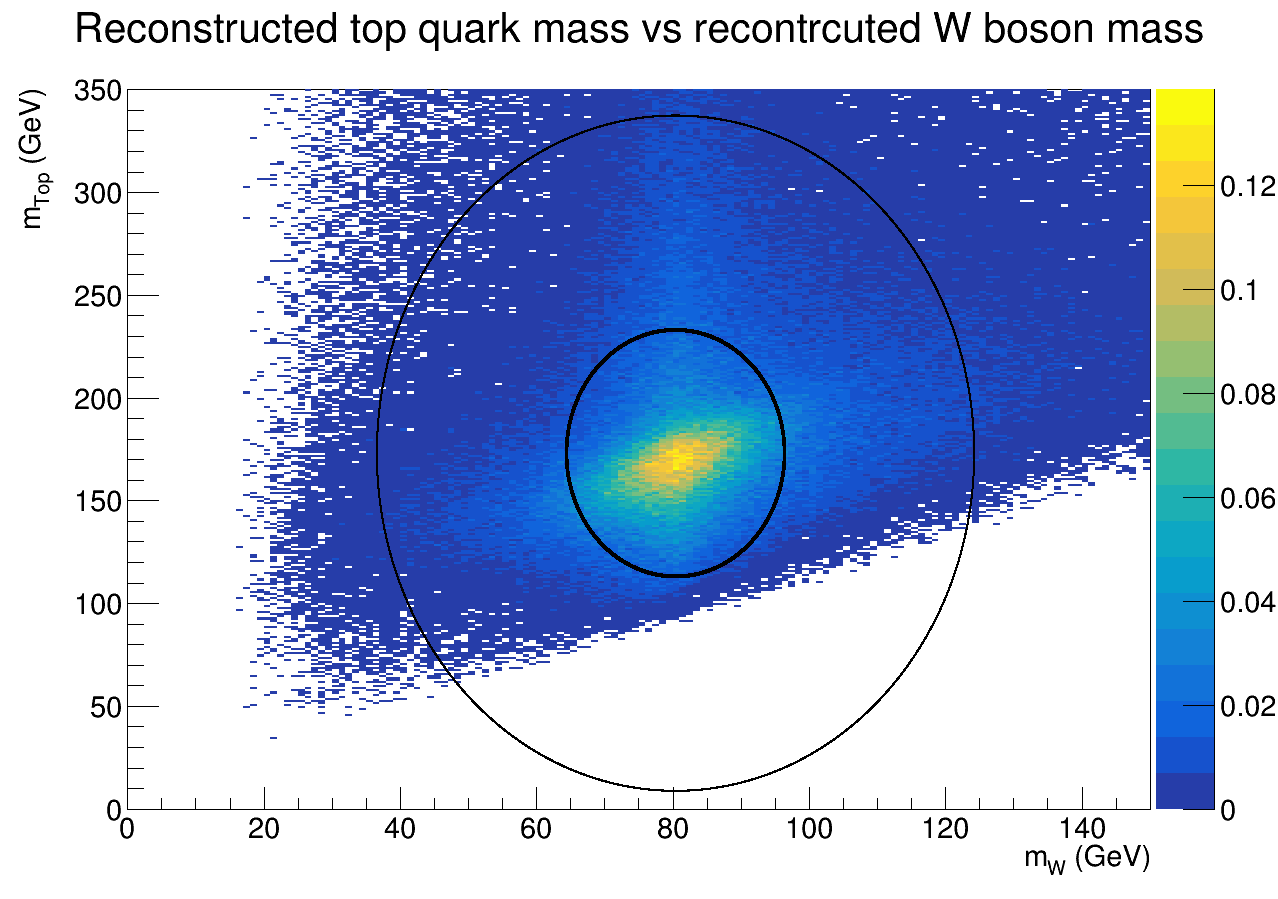
\includegraphics[width=0.49\textwidth]{figs/blinding/tZq_topVsWmass.png}
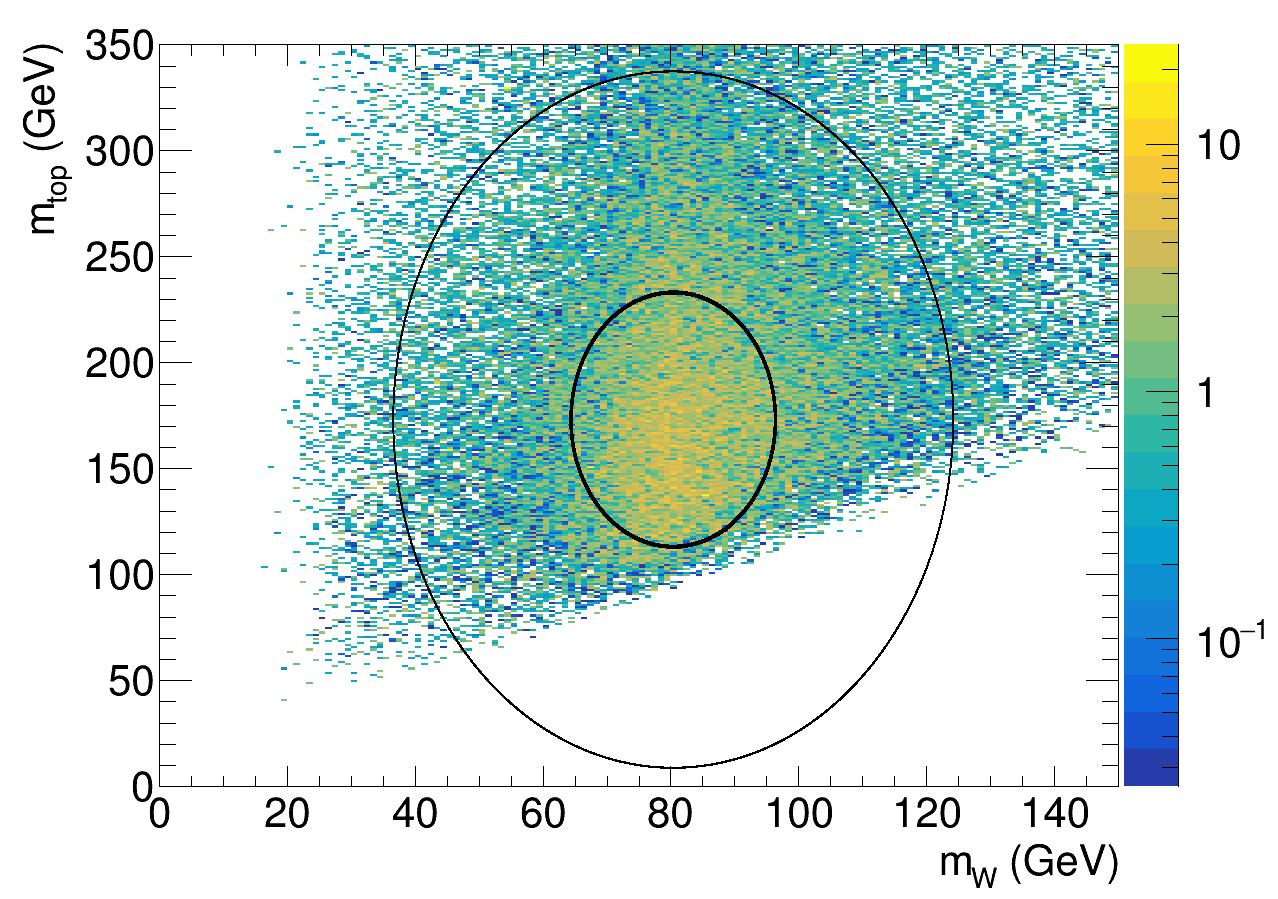
\includegraphics[width=0.49\textwidth]{figs/blinding/all_topVsWmass.png}
\caption{
The reconstructed top quark mass and w boson mass distributions for the tZq simulation sample (left) and all simulation samples (right) for both the $ee$ and $\mu\mu$ channels following the application of the signal region criteria described in Section~\ref{sec:signalRegion}.
The signal region is defined as the area within the inner contour line and the side-band region is defined as the are bounded between the two contour lines.
}
\label{fig:blindingChi2}
\end{figure}

\section{Trigger Strategy}\label{sec:triggerStrategy}
As the search for the tZq dilepton final state relies on the identification of the two leptons from the Z boson decay, the trigger strategy consists of selecting events from datasets identified by the triggering of an electron or muon trigger.
Given that the signal process being searched for is dominated by background processes and will likely be limited by event yield, it is essential to reconstruct and select as many signal events as possible.
To this end, in order to obtain the maximum event selection efficiency, events are required to have triggered a single lepton or a double lepton trigger for the $ee$ and $\mu\mu$ final states.

In simulation an event is required to pass either the single or double lepton triggers for the relevant channel.
In data however, there is the potential to double count events which are present in both the single lepton and double lepton datasets.
In order to avoid double counting events, events that have been found in a double lepton dataset are not considered for the single lepton dataset.
The trigger logic for each of the final states is illustrated in Table~\ref{tab:triggerCombo}.

\begin{table}[htbp]
\topcaption {
The trigger logic used for each of the CMS datasets considered, where \emph{EM} refers to the muon and electron triggers, \emph{EE} to the double electron triggers, \emph{E} to the single electron triggers, \emph{MM} to the double muon triggers, \emph{M} to the single muon triggers and \emph{!} to a trigger not being passed. 
}
\label{tab:triggerCombo}
  \centering
%  \resizebox{\textwidth}{!}{
   \begin{tabular}{ccc}
   \hline
   \textbf{Final State} & \textbf{Dataset} & \textbf{Trigger logic}  \\
   \hline
   \multirow{3}{*}{$e\mu$} & Muon and Electron & EM and !EE and !MM \\
   & Single Muon & M and !E and !EE and !MM and !EM \\
   & Single Electron & E and !M and !EE and !MM and !EM \\
   \hline
   \multirow{2}{*}{$\mu\mu$} & Double Muon & MM and !EM and !EE\\
   & Single Muon & M and !E and !EE and !MM and !EM \\
   \hline  
   \multirow{2}{*}{$ee$} & Double Electron & EE and !EM and !MM \\
   & Single Electron & E and !M and !EE and !MM and !EM \\
   \hline
 \end{tabular}%}
\end{table}

Ideally the, single and double lepton triggers with the lowest possible transverse momentum thresholds would be considered to ensure that the maximum possible event yield can be obtained over the largest possible phase space.
The high instantaneous luminosity at the start of the most luminous data taking periods, however, required a number of the L-1 triggers to be prescaled to prevent the trigger bandwidth constraints being exceeded.
As only the triggers considered for the $ee$ channel were impacted by this; these triggers were chosen on the basis of the amount of luminosity they were not prescaled for with the lowest possible transverse momenta thresholds.

Table~\ref{tab:triggersDatasets} lists the triggers used to select data and simulation events for each channel, including the e$\mu$ final state which is considered for a \ttbar enriched control region (see Section~\ref{subsec:ttbarCR}).
In these trigger path names, \emph{Ele} and \emph{Mu}, refer to a reconstructed electron and muon, respectively.
The number following the lepton flavour denotes the minimum \pT a lepton must have to fire the trigger.
In order to avoid raising \pT thresholds to maintain the trigger data rate, additional criteria are used by the triggers.
These include simple identification (\emph{Id}) and isolation (\emph{Iso}) criteria, which are extracted from the calorimeter (\emph{Calo}) and tracker (\emph{Trk}) systems, and filters to reject candidates that have not originated from the interaction point (\emph{DZ}).

\begin{table}[h]
\topcaption {
Triggers and datasets used for each decay channel.
}
\label{tab:triggersDatasets}
  \centering
   \resizebox{\textwidth}{!}{
   \begin{tabular}{ccc}
   \hline
   \textbf{Final State} & \textbf{Dataset} & \textbf{HLT Trigger Conditions}  \\
   \hline
    $ee$ & DoubleElectron & HLT\_Ele23\_Ele12\_CaloIdL\_TrackIdL\_IsoVL\_DZ \\
    & SingleElectron &  HLT\_Ele32\_eta2p1\_WPTight\_Gsf   \\
   \hline
    $\mu\mu$ & DoubleMuon  & HLT\_Mu17\_TrkIsoVVL\_(Tk)Mu8\_TrkIsoVVL(\_DZ) \\  
    & SingleMuon &  HLT\_Iso(Tk)Mu24  \\  
   \hline
   $e \mu$ & MuonEG &  HLT\_Mu12\_TrkIsoVVL\_Ele23\_CaloIdL\_TrackIdL\_IsoVL(\_DZ)   \\  
%          &        &  HLT\_Mu8\_TrkIsoVVL\_Ele23\_CaloIdL\_TrackIdL\_IsoVL(\_DZ)  \\
          &        &  HLT\_Mu23\_TrkIsoVVL\_Ele12\_CaloIdL\_TrackIdL\_IsoVL(\_DZ) \\
%    & SingleElectron &  HLT\_Ele32\_eta2p1\_WPTight\_Gsf   \\
%    & SingleMuon &  HLT\_Iso(Tk)Mu24  \\  
   \hline
 \end{tabular}}
\end{table}


\section{Event Cleaning}\label{sec:metFilters}
beam backgrounds/detector noises
After selecting an event that meets the trigger requirements described in Section~\ref{sec:triggerStrategy}, a number of filters are applied to remove events containing beam backgrounds or detector noise from further consideration:

\begin{itemize}
\item \textbf{Primary Vertex Filter:} Ensures that the primary vertex is well reconstructed by requiring it to be within $|z| \leq 24\cm$ of the interaction point and within $d_{0} < 2\cm$ of the beam line.
\item \textbf{Beam Halo Filter:} Beam halos are machine-induced particles (\ie produced from the beam interacting with the pipe and residual gas in the pipes) that circulate with the beam at radii of up to 5\cm. This filter removes events with calorimeter and muon chamber energy deposits consistent with those expected to be produced by either halo particles or particle showers.
These effects are caused by beam halos interacting with the collimator blocks that are used to clean halos from the beam.
\item \textbf{HBHE Noise and Isolation Filters:} Remove events where anomalous noise is observed in the HCAL's hybrid photodiodes or readout boxes, which registers as large isolated energy deposits which would infer the presence of large \MET, by considering the channel multiplicities, pulse shape of the readout and the neighbouring activity in the calorimeters and tracker.
\item \textbf{ECAL Trigger Primitive Filter:} The L-1 trigger primitive readout can be used to estimate the energy deposited in approximately 70\% of the channels that lack regular data links and which ignored in the offline reconstruction. As trigger primitives have a narrower energy acceptance range than the read-out, when the energy is near their saturation energy the measured energy is likely to be underestimated, resulting in high anomalous \MET. 
%\item \textbf{ECAL Endcap SC Filters} - NOT recommended for 2016
\item \textbf{Bad Charged Hadron Filter:} Removes events where a muon is not defined as a PF muon due to its low quality, but instead makes its way into the PF MET calculation as a mis-identified charged hadron candidate.
%\item \textbf{Bad Muon Filter} Removes events where a muon is defined as a PF muon, but still has too low a quality and large \pT to be considered.
\end{itemize}

\section{Physics Objects}\label{sec:physicsObjects}
In order select events consistent with the objects expected to be in the final states of the signal enriched region and background enriched control regions described in Sections~\ref{sec:signalRegion}-\ref{sec:controlRegions}, a number of event selection criteria are applied to the physics objects that have been reconstructed using the particle flow algorithm described in Chapter~\ref{chapter:data-mc}.
The following section describes the selection criteria used in this analysis and how the final state products are used to reconstruct their mother particles.

\subsection{Lepton Selection}
All PF electrons and muons identified by the PF algorithm must pass a set of kinematic requirements and a set of quality criteria defined by CMS.
The kinematic requirements are applied to ensure that the leptons lie fully within the detector's acceptance and that their transverse momentum lies in the region where the trigger is both fully efficient and well described in simulation.
The identification criteria have been designed to be efficient at selecting isolated leptons produced from W and Z boson decays and rejecting leptons that have been from decays from within jets or taus or from incorrectly reconstructed tracks.

Different ``working points'' (WPs) are determined for the set of variables used by each of identification criteria supported by the CMS Physics Object Groups.
The WPs are defined by their average selection efficiency in simulation, with the tighter WPs being less efficient, but having a lower misidentification rate.
For both electrons and muons  considered in the analysis, the ``tightest'' working point is used to select high purity collections of leptons, with the ``loosest'' working point used to veto events with any additional leptons.

\subsubsection{Electrons}\label{subsubsec:electronSelection}
For any PF electron candidate to be considered in the final analysis it must meet the following kinematic requirements:

\begin{itemize}
\item the \pt of the leading and subleading electrons considered must be greater than the 35\GeVc and 15\GeVc, respectively;
\item electrons must have $|\eta| \leq 2.50$ to ensure that the electrons are fully within the ECAL acceptance;
\item electrons with $1.4442 \leq \eta \leq 1.566$ are not considered as  accurate reconstruction cannot be undertaken in the transition region between the ECAL barrel and endcap;
\item the longitudinal impact parameter, $d_{z}$, of the electron must be less than 0.10\cm in the barrel and 0.20\cm in the endcap disks;
\item and the transverse impact parameter, $d_{xy}$, of the electron must be less than 0.05\cm in the barrel and 0.10\cm in the endcap disks.
\end{itemize}

The impact parameter cuts are applied to ensure that the electron originates from within the interaction point of the detector.

The \emph{tight} and \emph{veto} working points (WPs) of the CMS recommended electron identification criteria, which are approximately 70\% and 95\% efficient respectively, are used to select electrons and to veto any additional electrons.
This set of identification criteria uses a mixture of predetermined variables and multivariate analysis (MVA) tuned variables for both the barrel and endcap disks.
The values of the latter were set by the MVA determining the optimum values for a given selection efficiency, using simulated Z+jets and \ttbar+jets events as the signal and background processes respectively.

The predetermined variables are:
\begin{itemize}
\item \textbf{$N^{missing}_{inner hits}$:} As photons that subsequently convert into $e^{+} e^{-}$ pairs do not leave hits in the innermost layers of the tracker, electrons are rejected if the expected number of missing hits is exceeded.
\item \textbf{a conversion veto} - is applied for all working points. The photon to electron conversion veto tests if a pair of electron tracks originate from a common displaced vertex. Any electron which fails this criteria is rejected.
\end{itemize}

The MVA tuned variables include:
\begin{itemize}
\item \textbf{Full $5 \times 5 \sigma_{i\eta i\eta}$:} Describes the lateral extension of the shower along the $\eta$ direction, \ie the RMS alongside the $\eta$ direction inside the 5$\times$5 i$\eta$ tower.
\item \textbf{$\Delta \eta_{seed}$ and $\Delta \phi_{seed}$:} The distances in $\eta$ and $\phi$ between the ECAL supercluster and where the track has been extrapolated to from the primary vertex, respectively.
\item \textbf{$\frac{h}{E}$:} The ratio of hadronic to electromagnetic energy deposited in the supercluster around the crystal with the largest energy deposit.
\item \textbf{$I^{rel}_{EA}$:} The relative isolation of the electron with effective area pileup alleviation for a cone size of 0.3, which is described further in Section~\ref{subsubsec:relIso}.
\item \textbf{$1/E - 1/p$:} The difference between the inverse energy of the ECAL supercluster and the inverse of the track momentum, which is used to describe the energy loss of the electron due to material effects.
\end{itemize}

The selection requirements that define the tight and veto WPs for these variables are given in Table~\ref{tab:electronCuts}.

\begin{table}[htbp]
\topcaption {
The selection requirements used for the tight and veto working points of the cut based identification criteria for electrons for the barrel and endcap disks.
}
\label{tab:electronCuts}
  \centering
%  \resizebox{\textwidth}{!}{
% This right-aligns numbers in column, but centers them under column title.
 \begin{tabular}{ccccc}
   \hline
   \textbf{Variable} & \multicolumn{2}{c}{\textbf{Tight WP}} & \multicolumn{2}{c}{\textbf{Veto WP}}   \\
    & Barrel & Endcap & Barrel & Endcap \\
    \hline   
    Full $5\times5 \sigma_{i\eta i\eta}$ & $< 0.00998$ & $< 0.0292$ & $< 0.0115$ & $< 0.037$ \\
    $\Delta \eta_{seed}$ & $<0.00308$ & $<0.00605$ & $<0.00749$ & $<0.00895$ \\
    $\Delta \phi_{seed}$ & $<0.0816$ & $<0.0394$ & $<0.228$ & $<0.213$ \\
    $\frac{h}{E}$ & $<0.0414$ & $<0.0641$ & $<0.356$ & $<0.211$	\\
    $I^{rel}_{EA}$ & $<0.0588$ & $<0.0571$ & $<0.175$ & $<0.159$ \\
    $1/E - 1/p$ & $<0.0129$ & $<0.0129$ & $<0.299$ & $<0.15$ \\
    $N^{missing}_{inner hits}$ & $\leq 1$ & $\leq 1$ & $\leq 2$ & $\leq 3$ \\
    pass conversion veto & $\checkmark$ & $\checkmark$ & $\checkmark$ & $\checkmark$ \\
    \hline
 \end{tabular}%}
\end{table}

\subsubsection{Muons}\label{subsubsec:muonSelection}
PF muons are also required to meet an equivalent set of kinematic requirements along with identification and isolation criteria.

PF muons candidates are required to meet the following kinematic requirements:
\begin{itemize}
\item the \pt of the leading and subleading electrons considered must be greater than 26\GeVc and 20\GeVc, respectively;
\item muons must have $|\eta| \leq 2.40$ to ensure that a muon is fully within the acceptance of the muon systems.
\end{itemize}

The \emph{tight} and \emph{loose} identification and isolation criteria~\cite{Chatrchyan:2012xi} are used to select muons and veto any additional muons.

The tight muon criteria suppress hadronic punch-through into the muon system and selection of non-prompt muons, creating a high purity collection of particle flow muons.

These criteria are:
\begin{itemize}
\item As well as being identified as a PF Muon, it is also identified as both a tracker muon and global muon;
\item $\chi^{2}/ndf$ of the global muon track fit is less than ten;
\item at least one muon chamber is included in the global track fit;
\item that associated muon segments are found in at least two muon stations;
\item $d_{0} < 0.2\cm$ and $d_{z} < 0.5\cm$;
\item the muon must have at least one hit in the pixel detector.
\item the muon must have hits that are present in at least six tracker layers in order to achieve a good \pT measurement.
\end{itemize}

The tight muon isolation criteria applied to the resultant tight collection of muons is 95\% efficient and rejects muons that have a relative isolation greater than 0.15 for a cone size of 0.4.
By definition all PF muons considered pass the loose identification cut.
The loose isolation cut is 98\% efficient and rejects muons with a relative isolation that is greater than 0.25.
The $\Delta\beta$ pileup corrections used for relative isolation with muons is described below in Section~\ref{subsubsec:relIso}.

\subsubsection{Lepton Isolation}\label{subsubsec:relIso}
A relative isolation variable $I^{rel}$ is used in order to:
\begin{itemize}
\item differentiate between leptons produced promptly at the primary vertex from those resulting from heavy flavour jet or tau decays;
\item to ensure that leptons are sufficiently separated from hadrons and photons to enable a precise momentum measurement of the lepton .
\end{itemize}

$I^{rel}$ is defined as the summed energy of all PF particles within a cone of fixed radius $\Delta R$ around the PF lepton (with the estimated neutral charged pileup contamination, $\rho$, removed), divided by the lepton \pT.

As only charged hadrons ($CH$) have associated tracks that can be used to determine if they are consistent with the primary vertex, the pileup contamination contribution from neutral hadrons ($NH$) and photons is typically estimated using one of two methods.

In the analysis presented here,  the $\rho$ * effective area ($rho * A_{\rm eff}$) technique with a $\Delta R$ of 0.3 is used for the electron.
This method estimates the neutral pileup contributions by estimating and subtracting the median energy density per area of pileup contamination, $\rho$, which has been multiplied by the effective area of the electron, $A_{\rm eff}$.
This effective area is characterised as a function of the supercluster's $\eta$:

\begin{equation}
I^{rel}_{rho * A_{eff}} = \sum p_T(CH) + max (0.0, \sum E_{\rm T}(NH) + \sum E_{\rm T}(Photon) -\rho*A_{\rm eff} )/p_T \;
\end{equation}\label{eq:rhoEffA}

where the $max()$ function ensures that the corrected hadronic energy never negative.

The alternative $\Delta\beta$ pileup mitigation method is used for muons with a $\Delta R$ of 0.4 in the analysis presented here.
Using the fact that the ratio of neutral to charged hadron production in the hadronisation of pileup interactions is approximately 0.5, half of the transverse energy of charged hadrons from pileup is subtracted from the neutral hadron and photon transverse energies~\cite{Chatrchyan:2012vp}:

\begin{equation}
I^{rel}_{\Delta\beta} = \sum p_T(CH) + max (0.0, \sum E_{\rm T}(NH) + \sum E_{\rm T}(Photon) - 0.5 * \sum E_{\rm T}(PU))/p_T \;
\end{equation}\label{eq:deltaBeta}

\subsection{Jet, b-tagging, W Boson and Top Quark Candidate Requirements}
\subsubsection{Jet Requirements}
Jets belonging to the PF jet collection are considered, which are reconstructed using the \emph{anti-\kt} algorithm~\cite{Cacciari:2008gp} with R = 0.4 with charged hadrons originating from \PU vertices excluded from clustering.

Jets are considered in this analysis if they have a $\pT > 30\GeVc$, are within $|\eta| < 4.7$ and meet the \emph{loose} working point jet identification criteria developed by CMS.
The loose WP was chosen not only because it had a high selection efficiency and rejected the majority of the fake tracks, but also because the tight working point didn't increase the sensitivity of the search.
In addition, selected leptons (electron or muon) that lie within a cone of $\Delta R = 0.4$ of a selected jet are not considered to be a prompt leptons but are instead considered to be part of the jet in question.

The loose jet working point was designed to reject the majority of fake tracks produced within the detector and/or electronics noise. 
This working point maintains a high selection efficiency for real jets by requiring all jets to have part of their energy deposited in both the ECAL and HCAL and be composed of more than one particle.

For jets with $|\eta| \leq 2.70$, the loose working point criteria are:
\begin{itemize}
\item the fraction of the jet energy from both neutral electromagnetic particles in the ECAL and neutral hadronic particles in the HCAL is less than $0.99$.
\item the jet must consist of at least two particles.
\end{itemize}

The following criteria are additionally applied for jets for $|\eta| \leq 2.40$:
\begin{itemize}
\item the fraction of the jet energy from charged electromagnetic particles in the ECAL is less than $0.99$ and greater than 0.0 for charged hadronic particles in the HCAL.
\item at least one charged particle is present within the jet.
\end{itemize}

For jets with $ 2.70 \leq |\eta| \leq 3.0$ the loose working point criteria are:
\begin{itemize}
\item the fraction of the jet energy from neutral electromagnetic particles in the ECAL is greater than than $0.01$ and less than $0.98$ for neutral hadronic particles in the HCAL.
\item at least three neutral particles are present within the jet.
\end{itemize}

For jets with $|\eta| > 3.0$ the loose working point criteria are:
\begin{itemize}
\item the fraction of the jet energy in the ECAL that is from neutral electromagnetic particles is less than $0.90$.
\item at least eleven neutral particles are present within the jet.
\end{itemize}

\subsubsection{b-tagging Requirements}\label{subsubsec:bTag}
The CSVv2 tagging algorithm described in Section~\ref{subsec:objReco-bJets} is used to select jets that are deemed to have been initiated by a b-quark.
If the value of a jet's discriminator exceeds that of the Medium WP threshold and has $|\eta| < 2.40$, the jet is considered to be a b-jet.
Out of the \emph{Loose}, \emph{Medium} and \emph{Tight} WPs thresholds~\cite{Sirunyan:2017ezt} defined in Table~\ref{tab:bTagWPs} in Section~\ref{subsec:objReco-bJets}, the medium WP was selected.
This was because it provided the optimum performance in terms of providing as large a sample as possible for the signal process without too great a compromise on the purity of the selection.

\section{Background Processes}\label{sec:backgroundProcesses}
This next section discusses the background processes considered which can have the same final state as the signal process, their anticipated contributions to the background, and how they have been constrained.

The additional contributions from processes not considered here, where events that involve at least one jet that has been incorrectly reconstructed as a lepton or a lepton from the decay of a heavy quark, are discussed in Section~\ref{sec:NPLs}.

\subsection{Vector Boson in association with multijet backgrounds}
Multijet events in association with a vector boson have the largest cross sections of any process which produces prompt leptons at the LHC, as illustrated in Figure~\ref{fig:crossSections}.
As only one promptly produced lepton from the W boson decay is expected for W+jets, the presence of any additional leptons would have to be the result of a real heavy quark decay or fake reconstructed jet. 
Requiring any selected lepton to be sufficiently isolated from hadronic activity in the event will suppress the contribution from these events.

In contrast, while the Z+jets cross section is an order of magnitude smaller than the W+jets cross section, the two prompt leptons from the Z boson decay makes it much more difficult to distinguish between this background and the signal.
Despite requirement at least four jets, with at least one being a b-jet, in the signal region will reject the majority of the Z+jets events, the size of the Z+jets cross section ensures that the contribution from this process is still significant after all the selection criteria have been applied.

\subsection{Top physics backgrounds}
\ttbar has the next largest production cross section after W+jets and Z+jets.
While lepton isolation and jet cleaning criteria will significantly suppress the hadronic and lepton+jets final states, the dilepton final state provides the second largest background contribution when the two leptons that have been produced meet the Z boson selection criteria.

Similarly, the only single top production process anticipated to produce a significant background is the tW-channel when, due to gluon splitting and the two W bosons decaying leptonically, the final state that passes the event selection is indistinguishable from the \ttbar dilepton final state.
In contrast, negligible contributions are expected from the t- and s-channel processes
where no prompt leptons are produced in their respective final states after the event selection is applied.

While the processes where \ttbar is produced in association with a vector boson have cross sections many orders of magnitude smaller than \ttbar and single top production, only \ttbarZ where the Z boson decays leptonically is expected to be a significant background due to its indistinguishable topology from the signal process.
As the leading order final state has little to no expected \MET, jets from W boson decays, and six jets,
some of which may not be reconstructed due to merged or falling outside the detector acceptance, the vast majority of these events will pass the signal region criteria.
The lack of a real Z boson decay in \ttbarW, \ttbarH and tHq however, will result in the vast majority of events from these processes being rejected from consideration.

The rarest background considered is production of a single top quark in association with both a W and Z boson, tWZ.
While the dilepton final state of tWZ will be indistinguishable from the signal process, the tWZ cross section is an order of magnitude smaller than the tZq cross section.
Thus, this process, which also probes the top-W/Z couplings, will only contribute a very small number of events.

\subsection{Multi-boson backgrounds}
Multiple vector bosons produced through electroweak production form the remainder of the background processes considered.

Diboson processes involving the presence of a leptonically decaying Z boson and either a W or Z boson decaying hadronically with additional jets from gluon splitting were found to be the predominant source of background from these processes.
Smaller contributions from the other diboson final states are expected when multiple W bosons decay hadronically and/or jets are misreconstructed as leptons.
The tribosonic backgrounds form small contributions to the background due to their small production cross sections.